\chapter{L'intelligence artificelle aujourd'hui}
L'intelligence Artificelle est un domaine faisant partie 
des sciences cognitives dont l'objectif est de mettre au
point des techniques et technologies permettant aux 
machines de simuler l'intelligence humaine ou animale.
Nous pouvons séparer l'IA en deux catégorie distinctes. 

\section{Intelligence Artificielle Faible}
Elle reproduit un comportement de manière le plus précise possible,
en s'ameliorant notamment grâce à l'apprentissage 
mais n'en n'imite pas le fonctionnement ce qui fait que
ce type d'IA ne fait que simuler de l'intelligence. \newline
Aujourd'hui il n'existe que des intelligences artificelles faibles qui peuvent  
être séparées en plusieurs technique et sous-domaines \newline

\begin{figure}[!h]
    \centering
    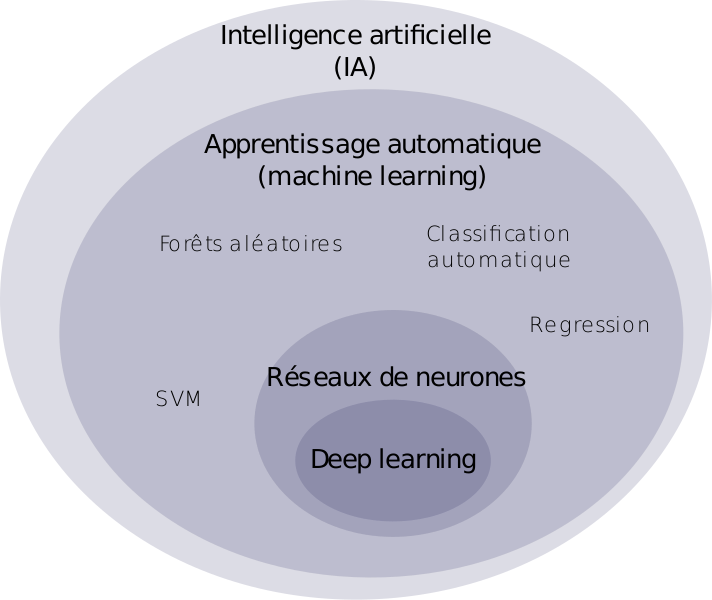
\includegraphics[width=0.8\textwidth]{Images/aitype}
    \caption{Les différents domaines de l'Intelligence Artificielle}
	\label{fig:categorieIA}
\end{figure}
\newpage

\subsection{Machine Learning}
Le Machine Learning est un ensemble de techniques qui permettent à un ordinateur 
d'agir et d'apprendre comme un humain tout en s'améliorant au fur et 
à mesure et ce de manière autonome. \newline

Le fonctionnement du machine learning ce découpe en plusieurs parties,
tout d'abord il faut définir des features, c'est à dire des
propriétés mesurables individuellement, cette partie est difficile et cruciale
car elle va déterminer l'efficacité de l'algorithme de machine learning. \newline

%je ne suis pas sur pour cette partie
Différents algorithme vont ensuite servir à extraire les features de données 
brut en entrée avant de les envoyer a l'algorithme de machine learning, par exemple 
la reconnaissance de bords ou de forme geométriques extraient les features d'une 
image dans une IA de reconnaissance d'image. \newline 

Enfin l'algorithme de machine learning va passer au travers de 3 sets de données:
\begin{itemize}
    \item un set de training va permettre d'entrainer l'algorithme de manière
     supervisé, ce set utilise des vecteurs d'entrée et leur sortie attendue.
    \item un set de validation qui va verifier le modèle crée à partir du set de 
    training.
    \item un set de test qui permet de tester la version finale de l'algorithme. 
\end{itemize}

\subsection{Deep Learning}
Le Deep Learning est une sous catégorie du machine learning, 
la différence majeur réside dans le fonctionnement du traitement des 
informations, le machine learning traditionnel ou "shallow", en contraste avec le deep learning,
réside dans la nécessité de selectionner manuellement les features qui doivent être 
identifiés par l'algorithme de machine learning:

\begin{figure}[!h]
    \centering
    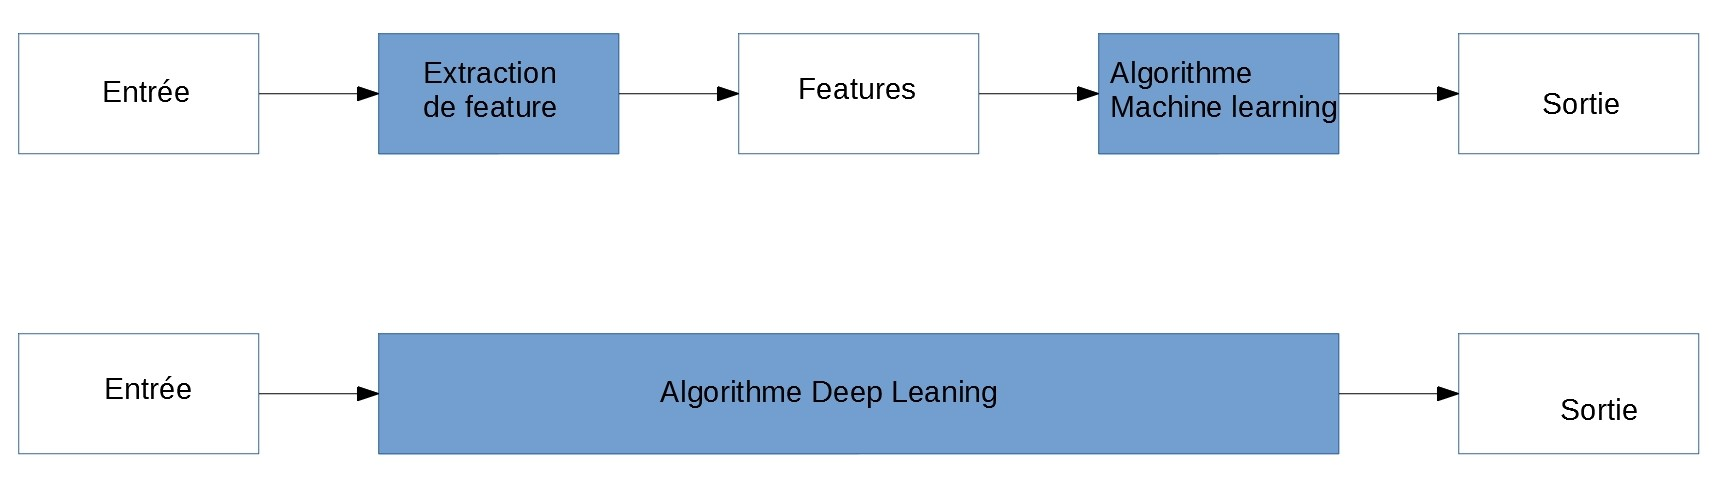
\includegraphics[width=1\textwidth]{Images/MLvsDL}
    \caption{Différences entre machine learning et deep learning}
	\label{fig:categorieIA}
\end{figure}

Le machine learning utilise des "réseaux de neurones", qui ont fait leurs premières 
apparition à partir de 1980, il s'agit de structure logiques imitant 
le comportement des neurones dans le cerveau humain, 
les neurones sont divisé en différentes couches: couche d'entrée, couche(s) cachée
et couche de sortie. 
\newpage

Dans le cas du "shallow" machine learning, le réseaux de neurones n'est composé 
qu'au maximum de 2 couches 

\begin{figure}[!h]
    \centering
    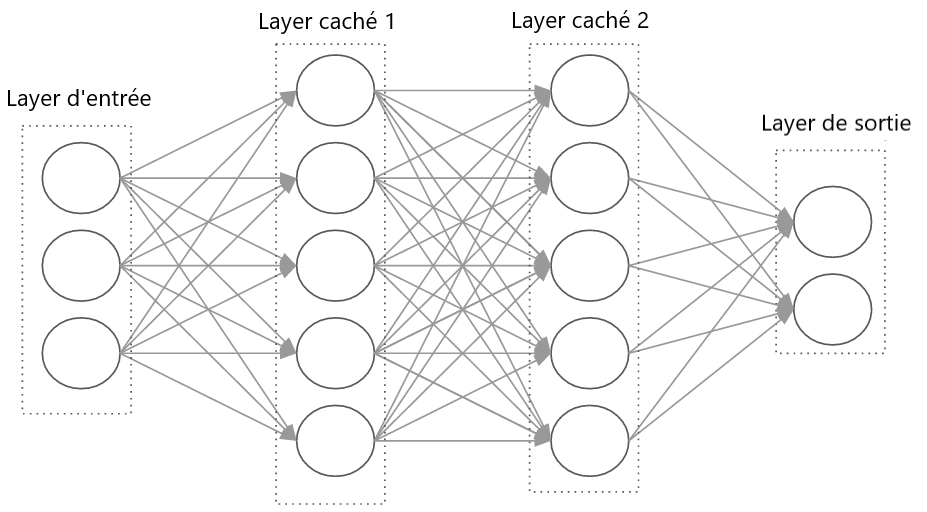
\includegraphics[width=1\textwidth]{Images/feedforward-nn}
    \caption{Réseau de neurones avec 2 couches cachées}
	\label{fig:categorieIA}
\end{figure}

%à mettre en fin ou en intro de la section ci-dessous ou à modifier
Du point de vue d'un observateur externe, l'IA faible
semble maitriser des concepts mais il n'en n'est rien dans la 
réalité, il suffit de reprendre l'exemple de la reconnaissance d'image
où comme l'IA ne comprend pas les concept et ne peut reconnaitre 
que des éléments correspondant au critères avec lequels elle a été 
entrainé, si on lui présente un élément avec une variance elle 
sera incapable de le reconnaitre.

\newpage
\section{Intelligence Artificielle Forte}
L'intelligence artificelle forte est l'intelligence
telle qu'elle existe chez l'homme, 

%apres l'explication il faut montrer quelques cas d'utilisation
%en situation réelle de ces technos je pense 




